\section{RISC Architecture}
\label{ch:arch}
An architecture describes a computer as seen by the programmer and the compiler designer. It
specifies the resources, i.e. the registers and memory and defines the instruction set. (possibly
implying data types).

Processors consist of two parts, the \emph{arithmetic/logic unit} (ALU) and the \emph{control unit} (CU).
The former performs arithmetic and logical operations, the latter controls the flow of operations. In
addition to the processor there is memory. Our RISC consists of a memory whose individually addressable
elements are bytes (8 bits).

The ALU features a bank of 16 registers with 32 bits. 32-bit quantities are called words. AL operations,
represented by instructions, always operate on these registers. Data can be transferred between memory
and registers by separate \emph{load} and \emph{store} instructions. This is an important characteristic
of RISC architectures, developed between 1975 and 1985. It contrasts with the earlier CISC (Complex ISC)
architectures: \emph{Memory is largely decoupled from the processor}. A 2nd important characteristic is
that \emph{every instruction takes one clock cycle for its execution}, perhaps with the exception of
access to slower memory. More about this will be presented later. This single-cycle rule makes such
processors predictable in performance. The number of cycles and the time required for executing any
instruction sequence is precisely defined. Predictability is essential in all real-time applications.

The core of the data processing unit consisting of ALU and registers is shown in Figure \ref{fig:alu}.
Evidently, data cycle
\begin{figure}
  \centering
  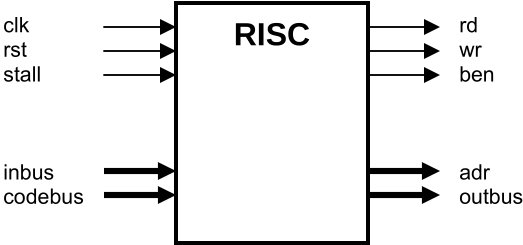
\includegraphics[width=.6\textwidth]{i/1.png}
  \caption{Processor core with ALU and registers}
  \label{fig:alu}
\end{figure}
from registers into the ALU, where an operation is performed, and the result is deposited back into a register.

The CU contains an \emph{Instruction Register} (IR) holding the instruction currently being under execution.
It also features a traditionally called \emph{Program Counter} (PC) register, holding the address of the
instruction being fetched from program memory. The CU computes the address of the next instruction. As this
is mostly the one in sequence, i.e. with address $PC+1$, the CU also holds an incrementer. Branch instructions
take the next address from IR.

External devices are mapped into the address space of memory. This means that a certain range of
addresses is reserved for access to input and output devices.
